\section{Game Overview \& Major Concepts}

Wheel of Elements is a cooperative Card Battler and Deckbuilder for 3 to 5 players. Sculpt your deck, find unexpected synergies, fight hordes of enemies and see them dance around the wheel.

\begin{minipage}[t][5cm][t]{1\textwidth}
	\begin{minipage}[t][5cm][t]{0.45\textwidth}
	\subsection*{Objective} - To win the game you must form a party of heroes and vanquish all enemies from the story you choose to play. You will be defeated if all players reach 0 hp. Some of you may die, but  that is a sacrifice you should be willing to make.\\
	\end{minipage}
	\hspace{0.05\textwidth}
	\begin{minipage}[t][5cm][t]{0.5\textwidth}
			\centering
			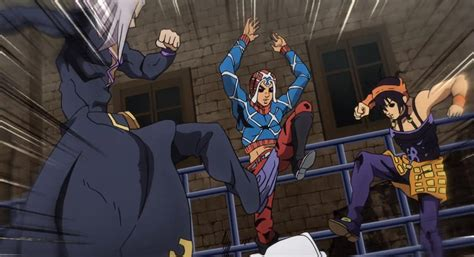
\includegraphics[width=\linewidth, valign=t]{../PicsRaw/JojoRef.jpg}
		%\end{figure}
		
		%\fbox{\parbox[4cm]{\textwidth}{Jojo-reference to people kicking one downed guy, but its players vs one enemy}}
	\end{minipage}
\end{minipage}

\begin{minipage}[t][5cm][t]{1\textwidth}
	\begin{minipage}[t][5cm][t]{0.45\textwidth}
		\fbox{\parbox[4cm]{\textwidth}{Picture of one action card, and possibly enemy actions with arrows back and forth}}
	\end{minipage}
	\hspace{0.05\textwidth}
	\begin{minipage}[t][5cm][t]{0.5\textwidth}
		\subsection*{Combat} - During Combat you will have to carefully manage your health while fighting of your enemies. The enemies revolve around the Wheel of Elements, and choose their attacks based on the current element facing towards them. \\
	\end{minipage}
\end{minipage}

\begin{minipage}[t][5cm][t]{1\textwidth}
	\begin{minipage}[t][5cm][t]{0.45\textwidth}
		\subsection*{The Wheel of Elements} - The (physically) central object is the Wheel of Elements. On it you track the state of the elements - a shared resource that all players generate and consume together. Coordinating large quantities of elements lets you play cards far stronger than any one player could wield on their own.\\
	\end{minipage}
	\hspace{0.05\textwidth}
	\begin{minipage}[t][5cm][t]{0.5\textwidth}
		\fbox{\parbox[4cm]{\textwidth}{The wheel}}
	\end{minipage}
\end{minipage}

\begin{minipage}[t][5cm][t]{\textwidth}
	\subsection*{Game Structure}
	\centering
	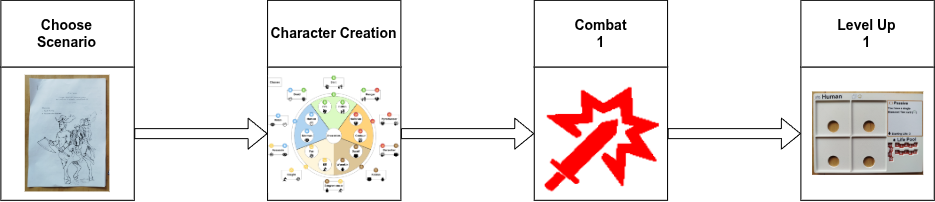
\includegraphics[width=\linewidth, valign=t]{../ExplanationPics/GameStructureLeft.drawio.png}
	%\end{figure}
\end{minipage}


\newpage

\begin{minipage}[t][5cm][t]{1\textwidth}
	\begin{minipage}[t][5cm][t]{0.45\textwidth}
		\subsection*{Multiclassing} - To form the characters you play as, you will pick one ancestry giving you a large twist on the gameplay, and multiple classes which determine the specifics of your strategy. With each of these decisions you will be granted a passive effect and cards for your deck. The vast options will let you explore many strategies and let you put your own favourite spins on them.\\
	\end{minipage}
	\hspace{0.05\textwidth}
	\begin{minipage}[t][5cm][t]{0.5\textwidth}
		\fbox{\parbox[4cm]{\textwidth}{One ancestry Tableau and many class tiles in the motion of getting placed into the tableau}}
	\end{minipage}
\end{minipage}


\begin{minipage}[t][5cm][t]{1\textwidth}
	\begin{minipage}[t][5cm][t]{0.45\textwidth}
		\fbox{\parbox[4cm]{\textwidth}{Sample cards, going in and out of a deck}}
	\end{minipage}
	\hspace{0.05\textwidth}
	\begin{minipage}[t][5cm][t]{0.5\textwidth}
		\subsection*{Deckbuilder} - The choices in ancestries and classes you make in the beginning will grant you your first deck of cards. With every new choice of class, you will gain new cards into the pool of cards you can choose from. For each encounter onward, you will then choose the cards which you include in your deck, and which you want to leave out. \\
	\end{minipage}
\end{minipage}



\begin{minipage}[t][5cm][t]{1\textwidth}
	\begin{minipage}[t][5cm][t]{0.45\textwidth}
		\subsection*{Co-operative} - You are playing together as one team. Whether win or loose you do it together.  You may talk and coordinate to get where you want.\\
	\end{minipage}
	\hspace{0.05\textwidth}
	\begin{minipage}[t][5cm][t]{0.5\textwidth}
		\fbox{\parbox[4cm]{\textwidth}{People, running around together and frolicking}}
	\end{minipage}
\end{minipage}

\begin{minipage}[t][5cm][t]{\textwidth}
	\vspace{2.5cm}
	\centering
	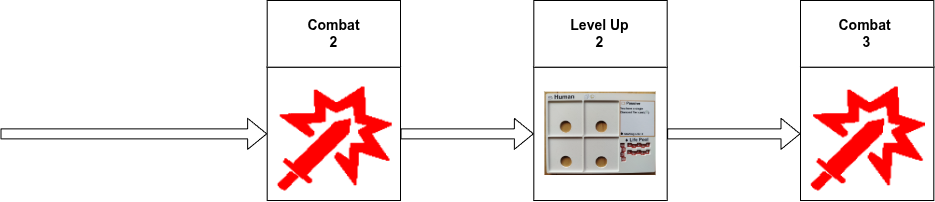
\includegraphics[width=\linewidth, valign=t]{../ExplanationPics/GameStructureRight.drawio.png}
	%\end{figure}
\end{minipage}